% Include from Manuscript/main.tex with % Include from Manuscript/main.tex with % Include from Manuscript/main.tex with % Include from Manuscript/main.tex with \input{content_profiles/figures}.
% Requires \usepackage{graphicx}. Descriptive synthesis of archived extraction.
\begin{figure}[p]
  \centering
  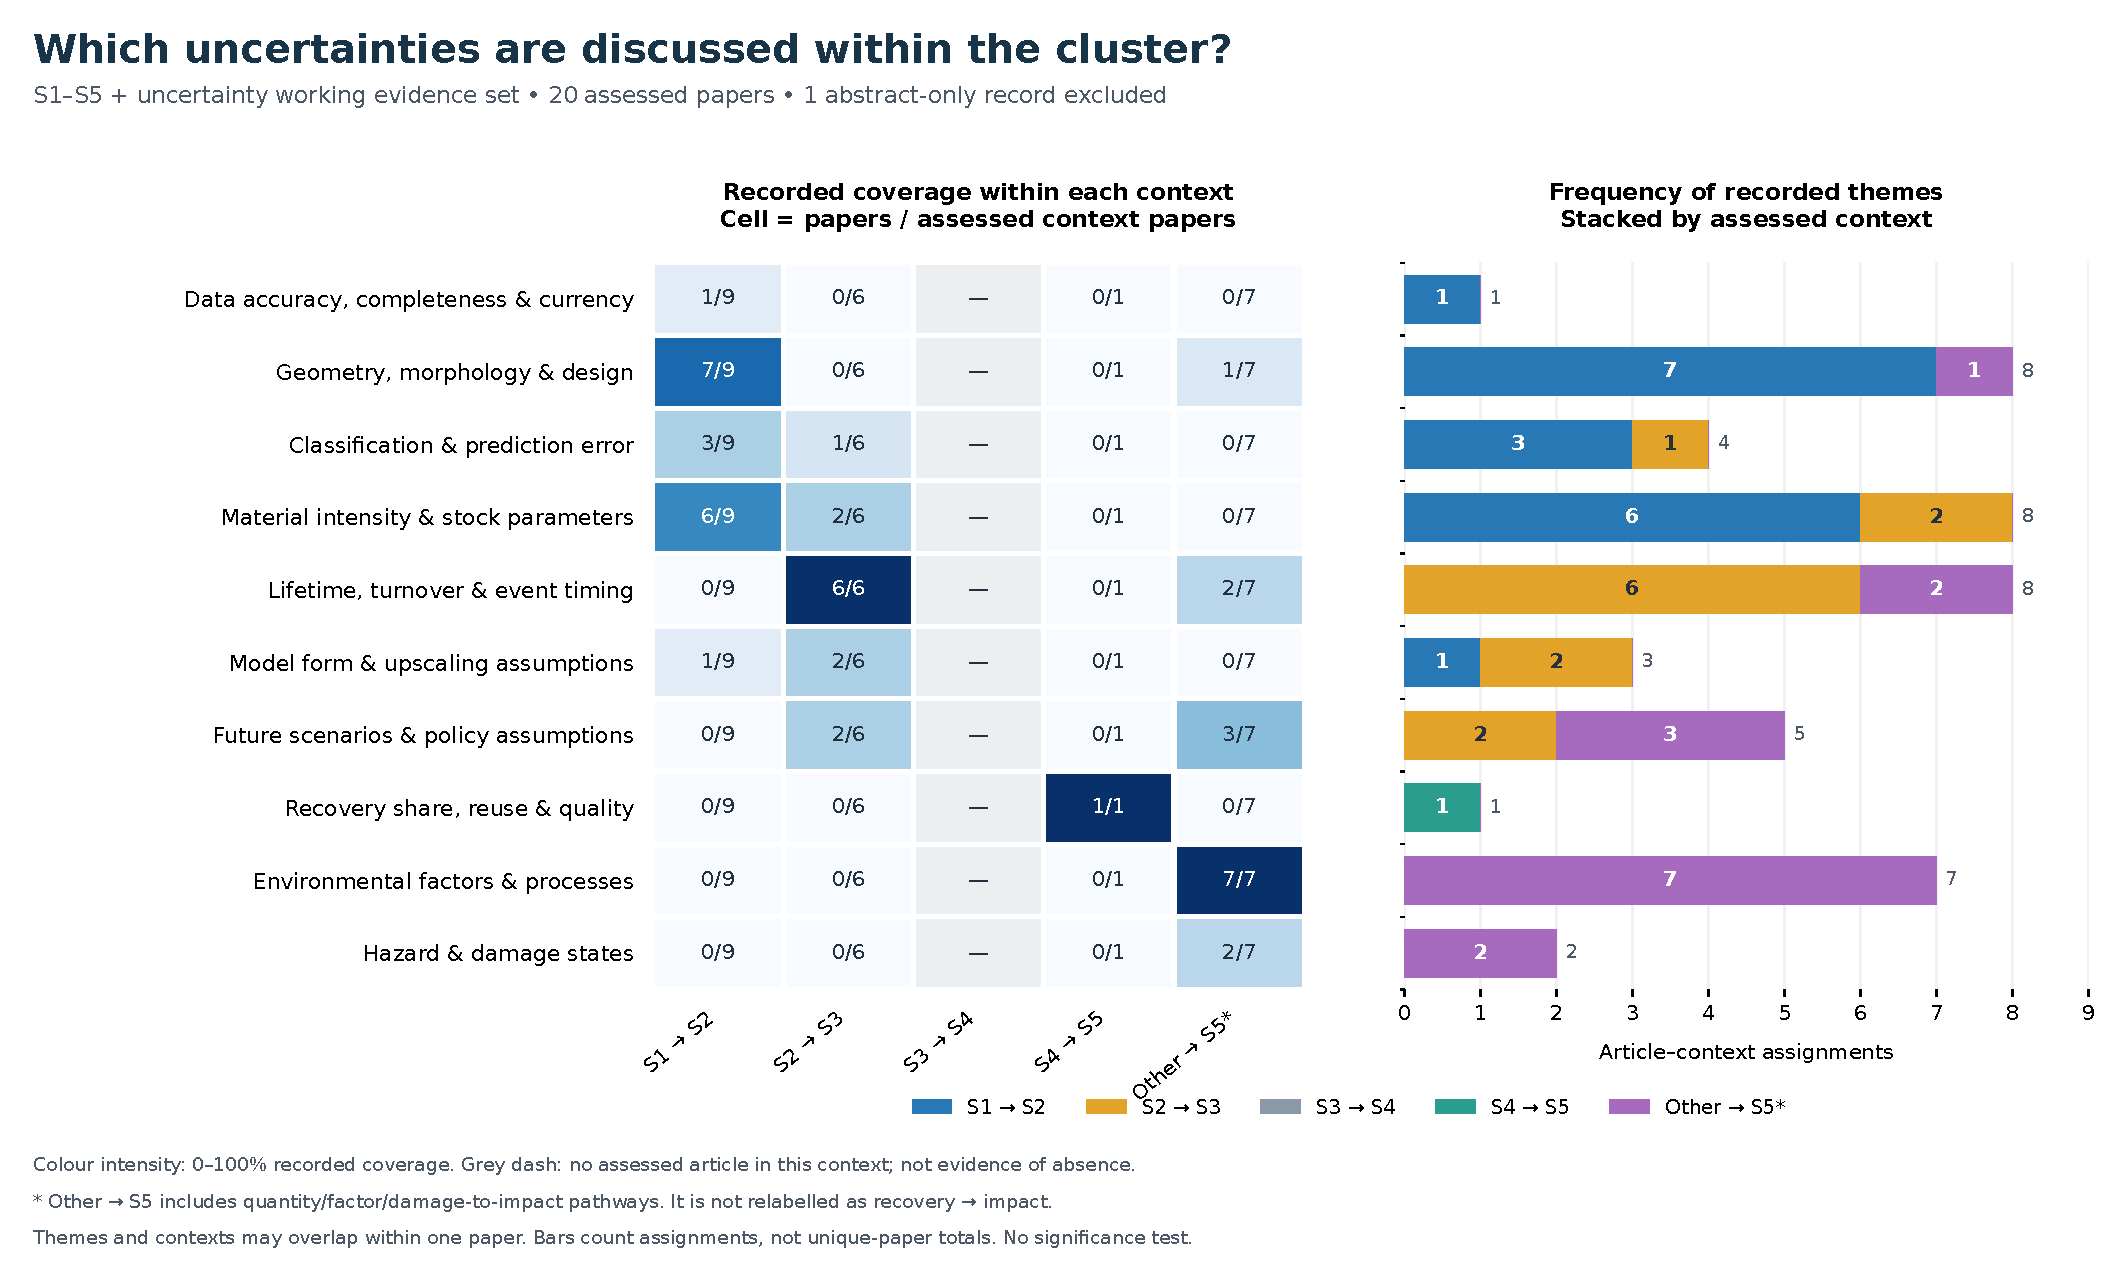
\includegraphics[width=\textwidth]{content_profiles/figures/01_uncertainty_sources.pdf}
  \caption{Recorded uncertainty sources within the S1--S5 uncertainty working set. Cells show papers with a recorded theme divided by assessed papers in each transition context. Twenty papers yield 23 article--context assessments; an abstract-only record is excluded. Themes and contexts may overlap. The grey column denotes no assessed article, not absence in the wider literature. The other-to-S5 group includes factor-, quantity- and damage-to-impact pathways and must not be interpreted as recovery-to-impact evidence.}
  \label{fig:content-uncertainty-sources}
\end{figure}

\begin{figure}[p]
  \centering
  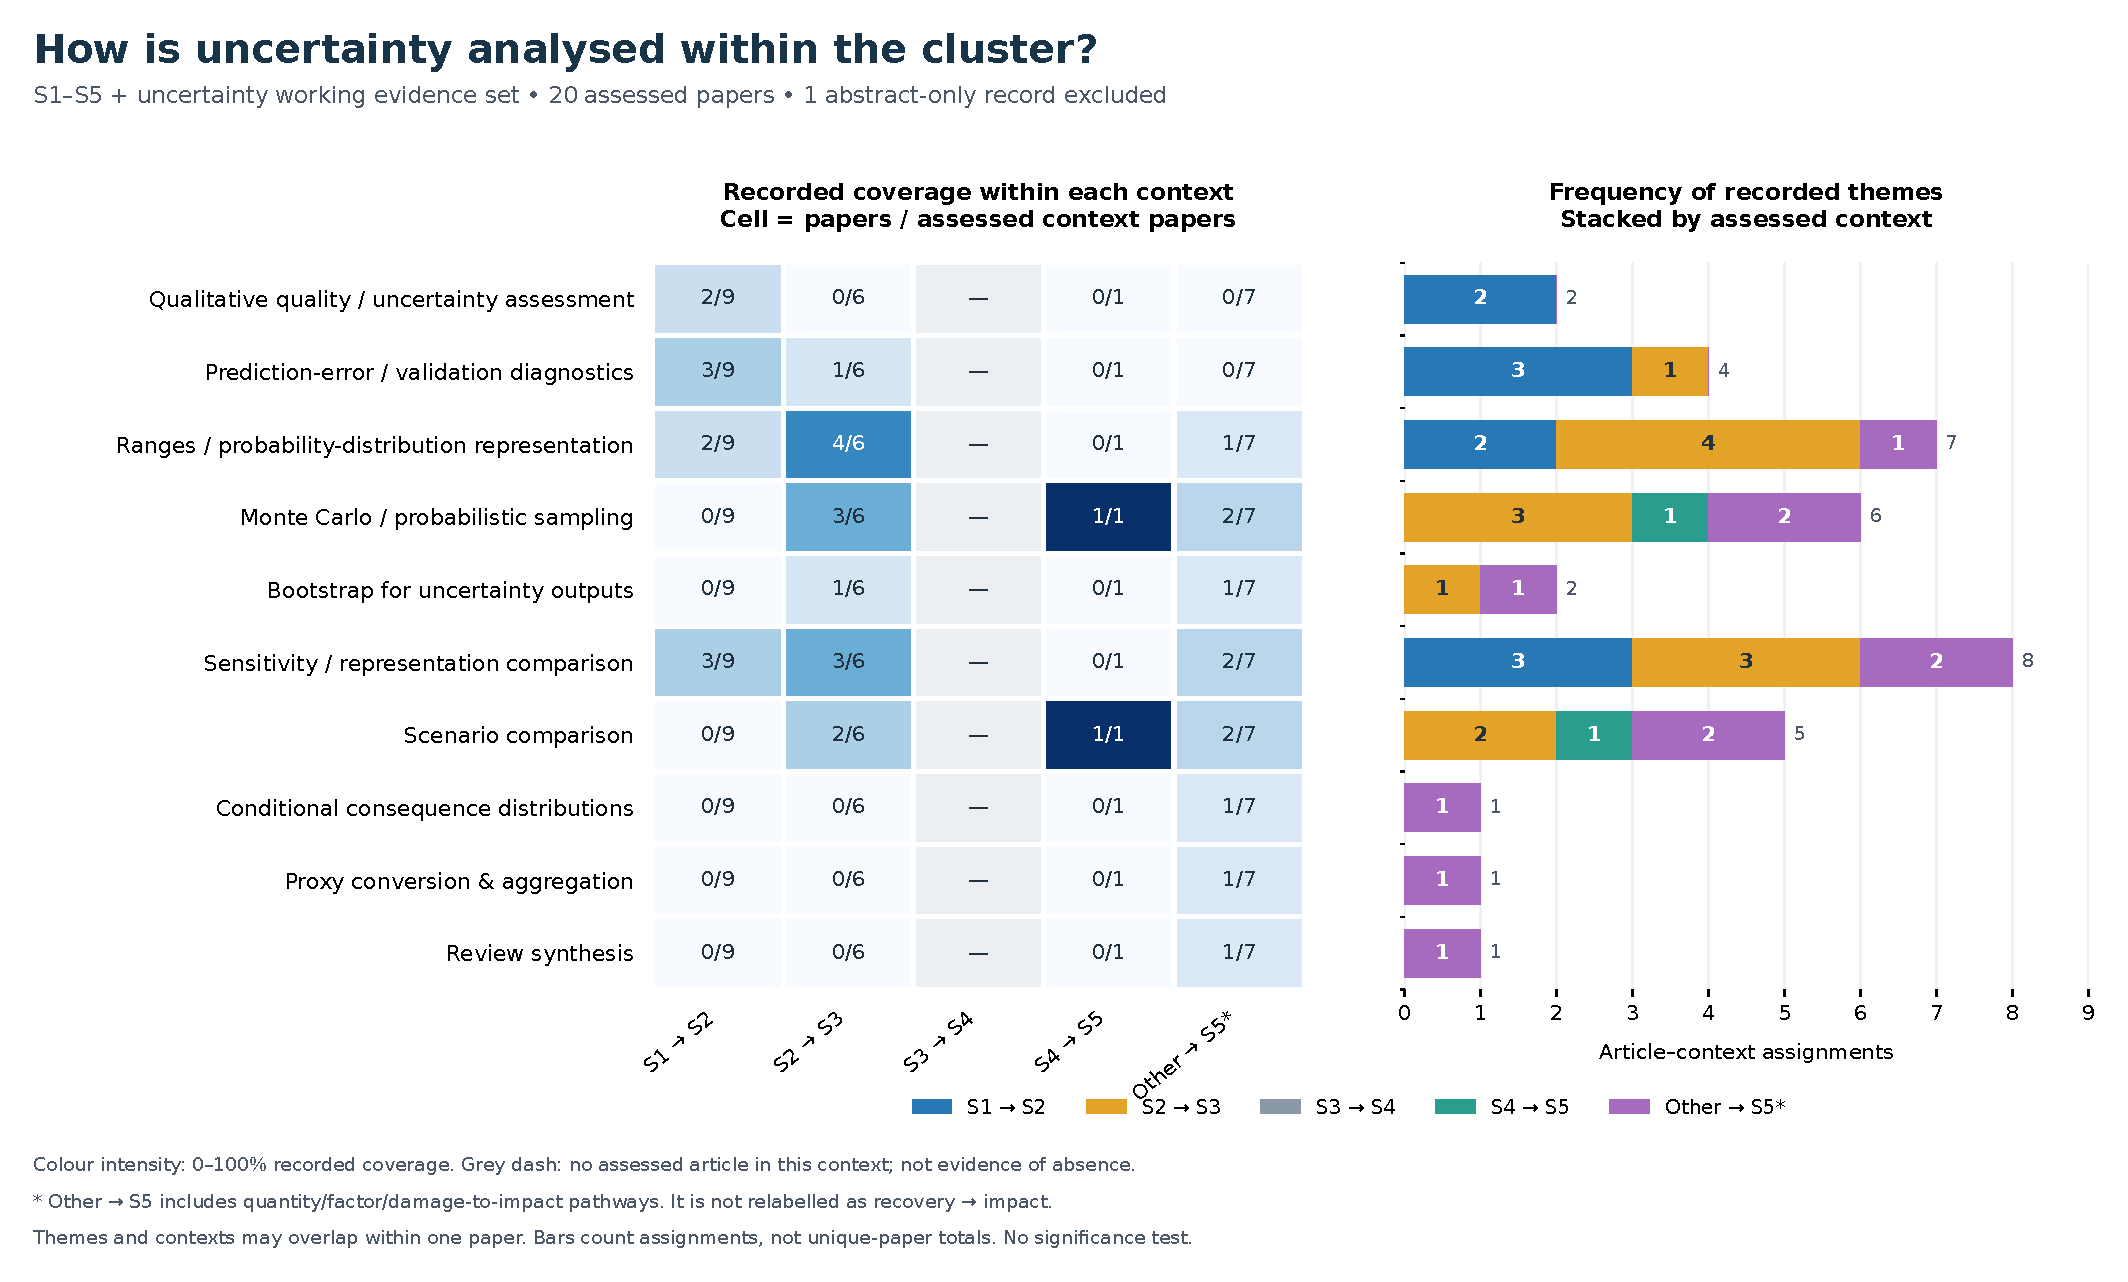
\includegraphics[width=\textwidth]{content_profiles/figures/02_uncertainty_methods.pdf}
  \caption{Recorded uncertainty-analysis methods in the same working set. Heatmap intensities are descriptive within-context proportions. Stacked frequencies count article--context assignments, not independent observations or unique-paper totals. A method's presence does not establish interstage uncertainty continuity. No inferential significance test is applied.}
  \label{fig:content-uncertainty-methods}
\end{figure}

\begin{figure}[p]
  \centering
  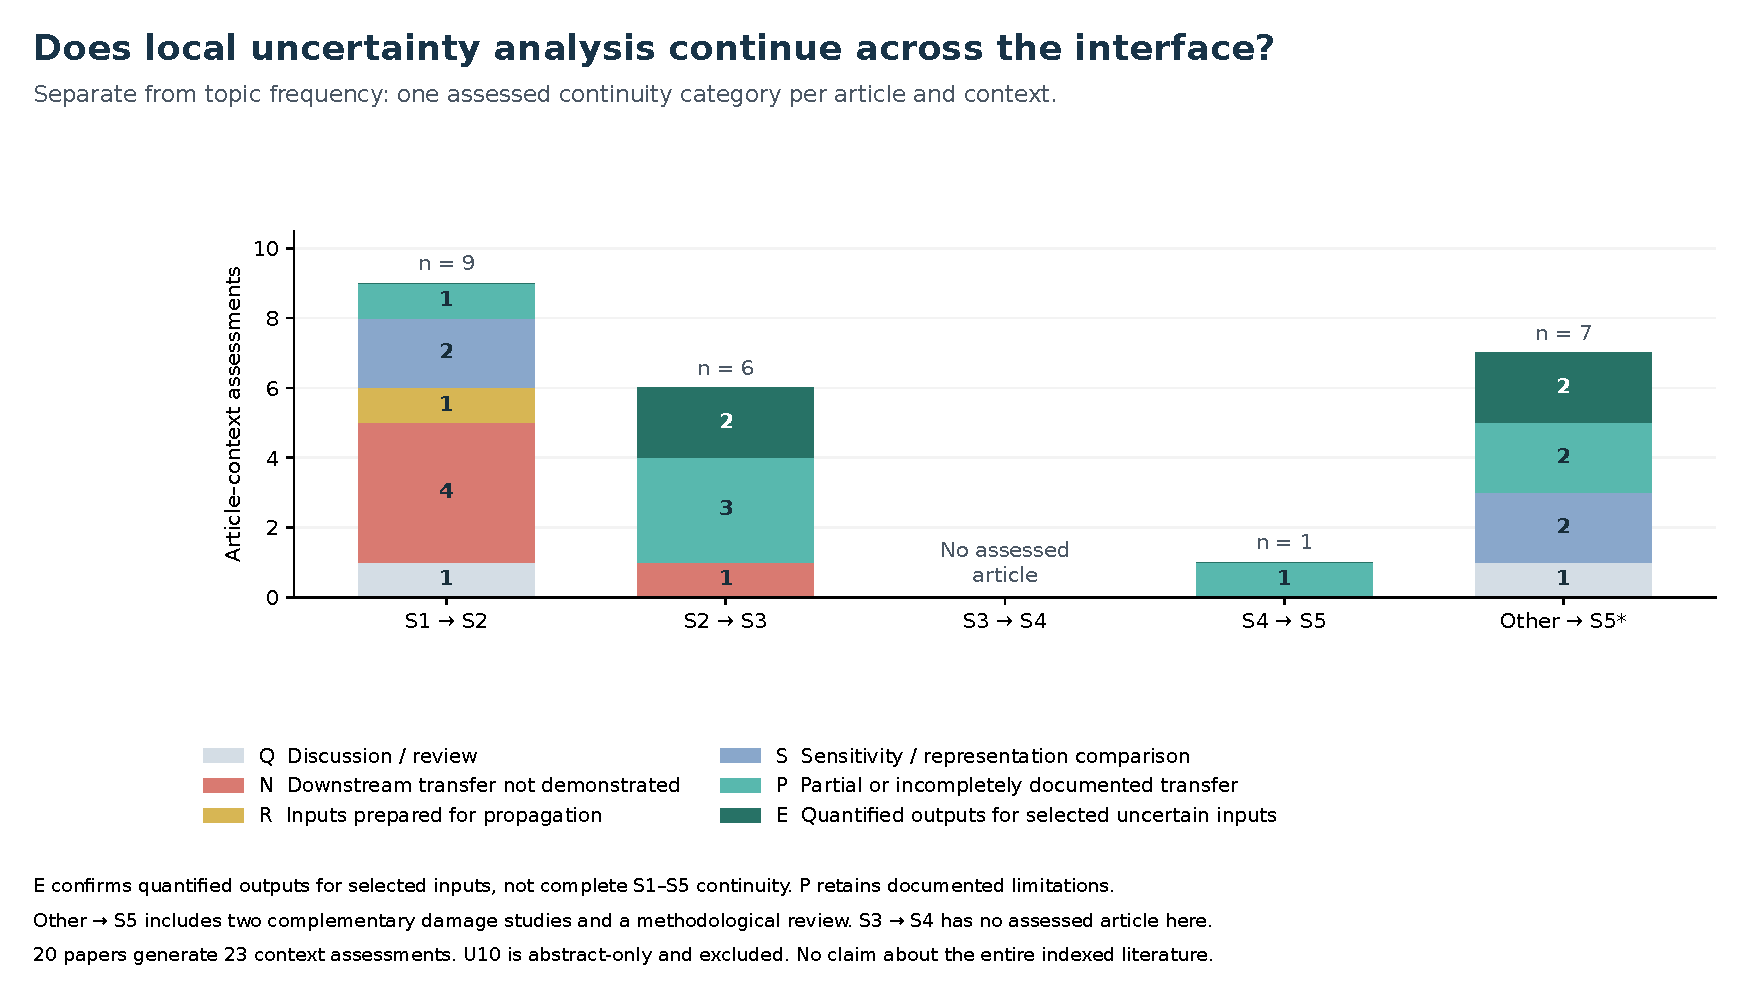
\includegraphics[width=\textwidth]{content_profiles/figures/03_continuity_evidence.pdf}
  \caption{Context-specific continuity assessments derived from archived evidence extraction. Each article--context pair has one assessment category. Quantified outputs for selected uncertain inputs do not demonstrate complete S1--S5 continuity. Methodological and complementary evidence retain their separate roles in the accompanying CSV. This figure does not constitute a new independent full-text review or a final PRISMA inclusion count.}
  \label{fig:content-continuity}
\end{figure}
.
% Requires \usepackage{graphicx}. Descriptive synthesis of archived extraction.
\begin{figure}[p]
  \centering
  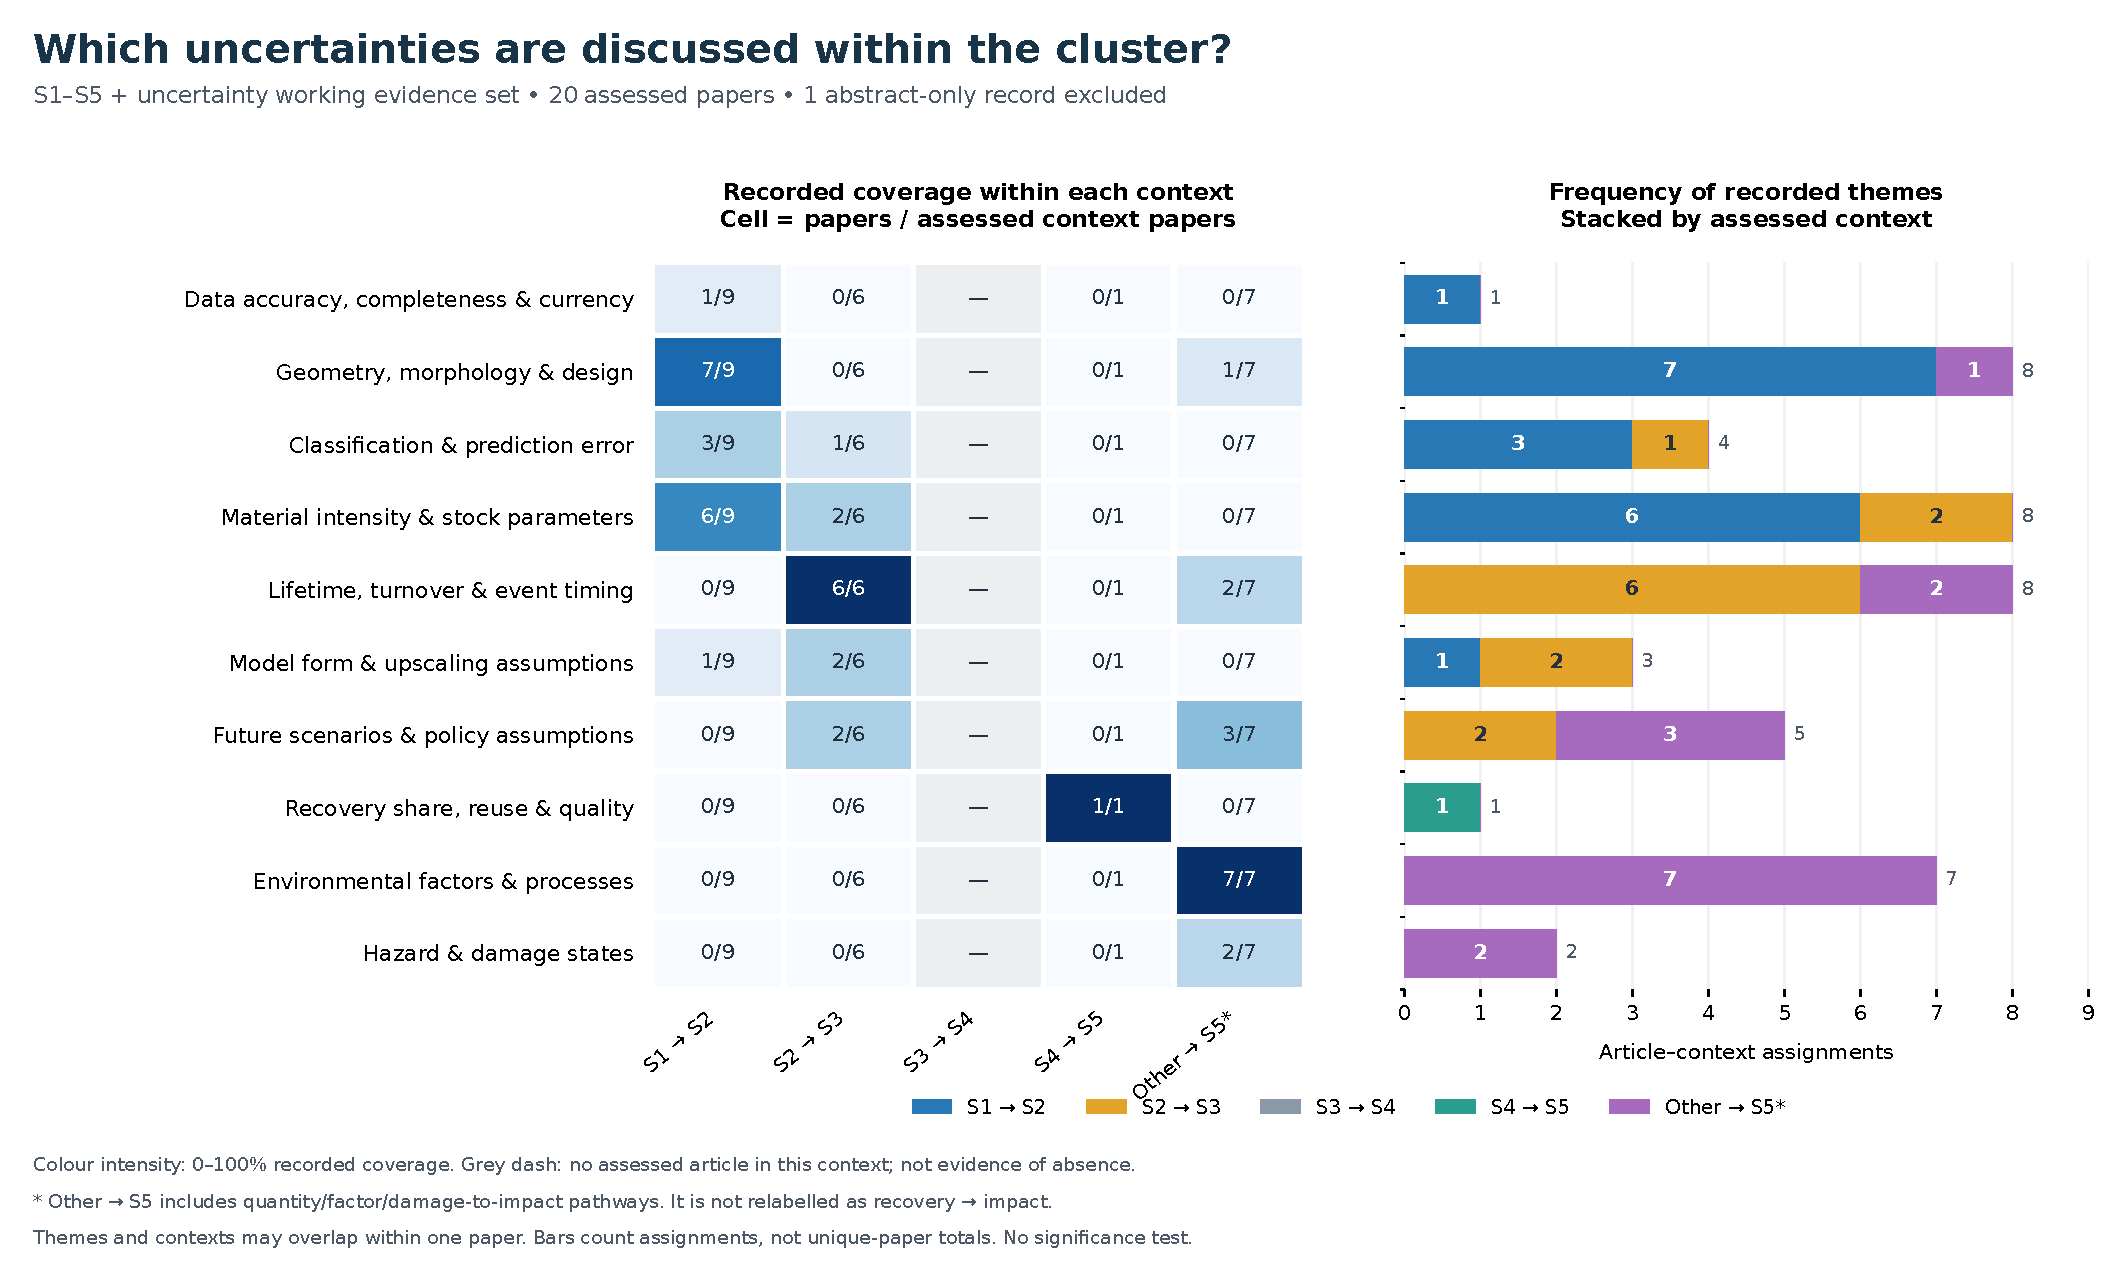
\includegraphics[width=\textwidth]{content_profiles/figures/01_uncertainty_sources.pdf}
  \caption{Recorded uncertainty sources within the S1--S5 uncertainty working set. Cells show papers with a recorded theme divided by assessed papers in each transition context. Twenty papers yield 23 article--context assessments; an abstract-only record is excluded. Themes and contexts may overlap. The grey column denotes no assessed article, not absence in the wider literature. The other-to-S5 group includes factor-, quantity- and damage-to-impact pathways and must not be interpreted as recovery-to-impact evidence.}
  \label{fig:content-uncertainty-sources}
\end{figure}

\begin{figure}[p]
  \centering
  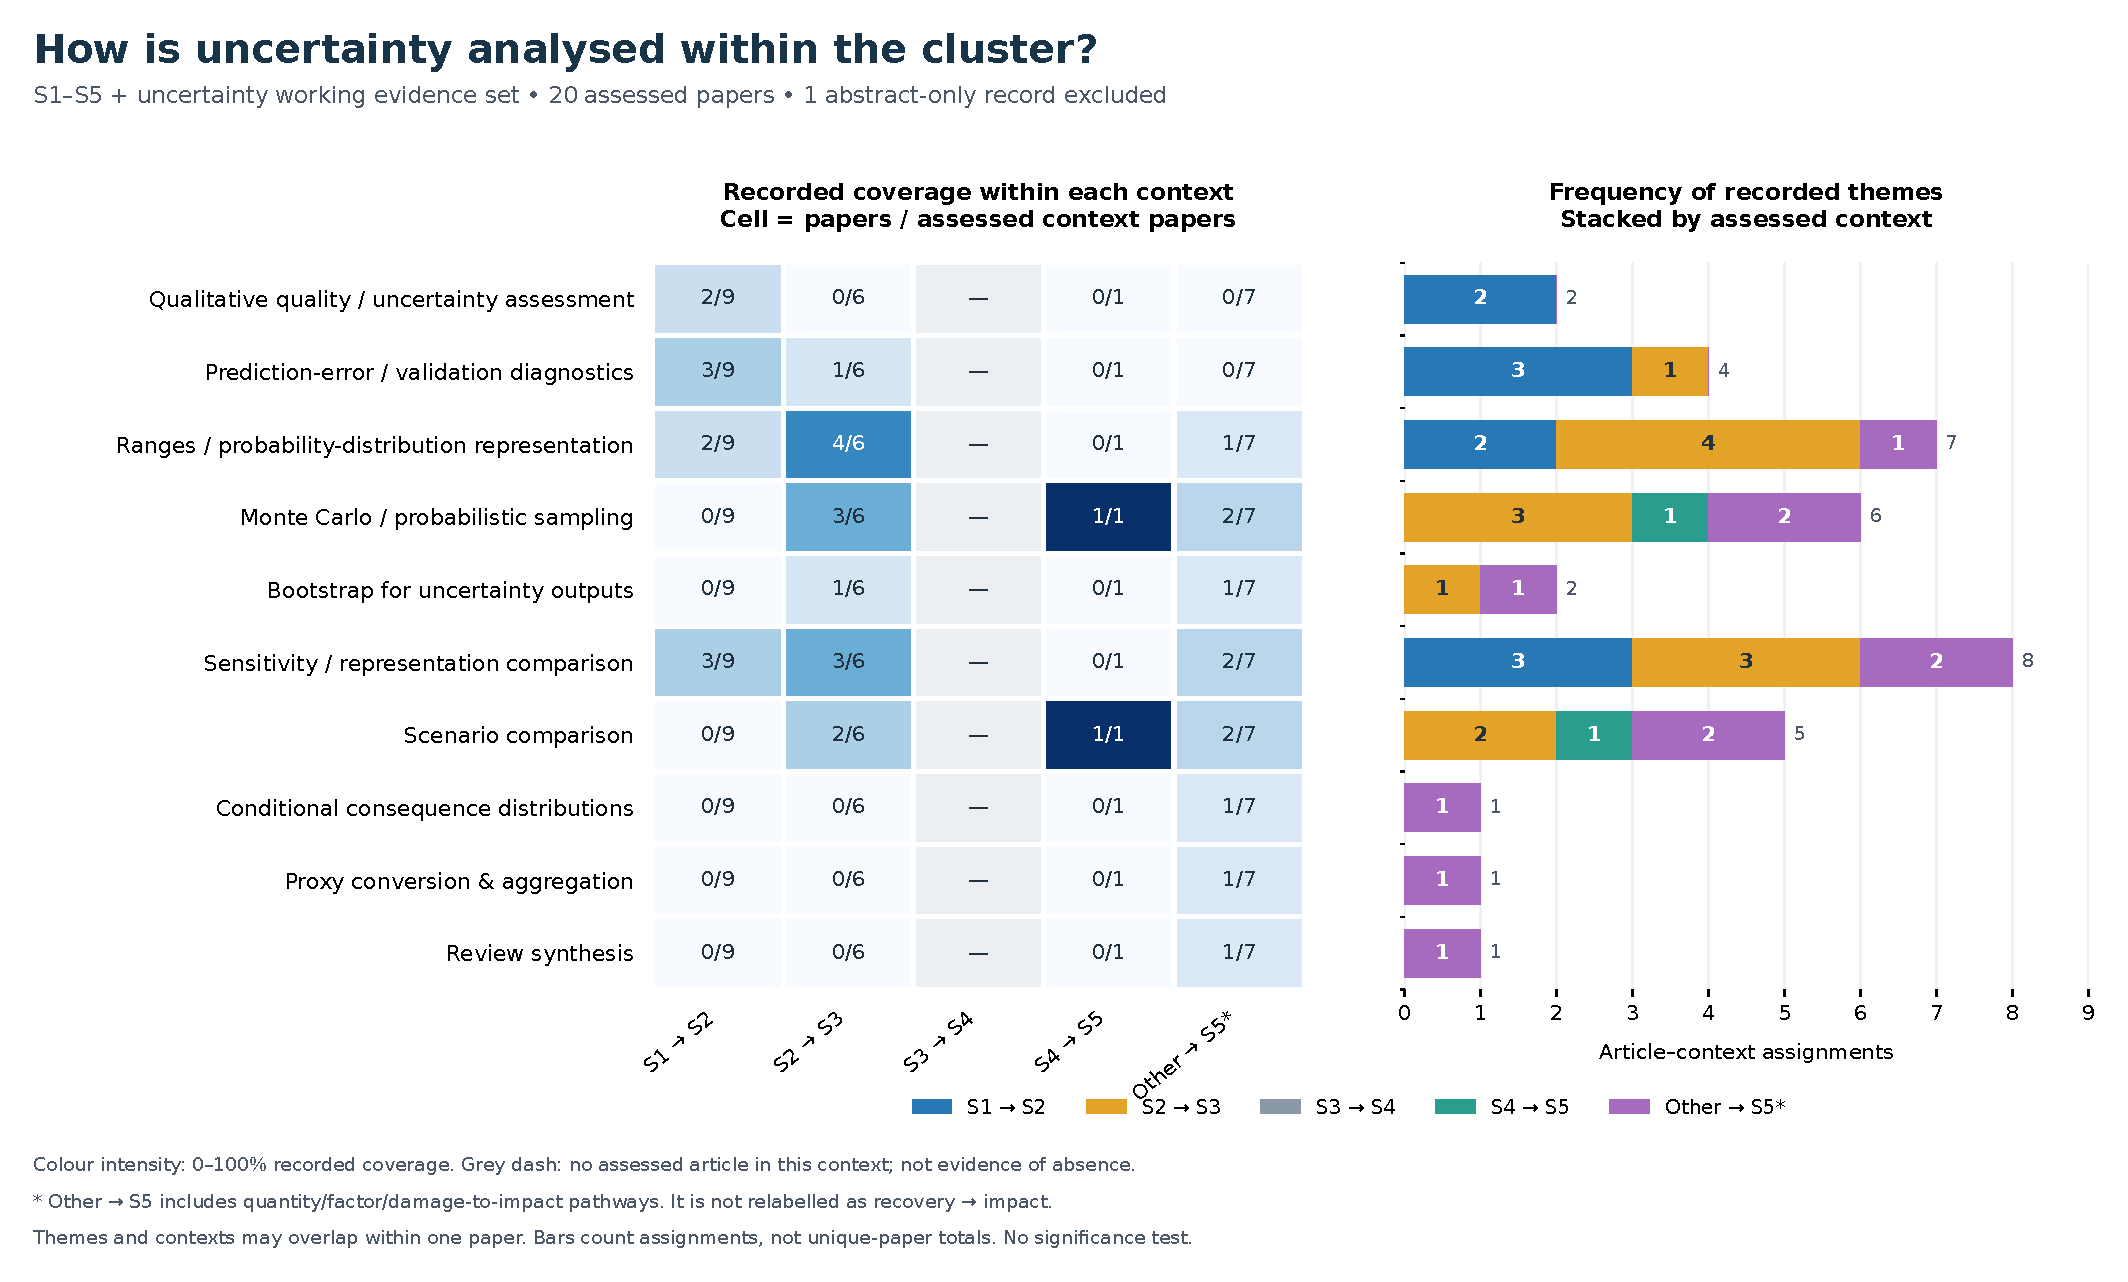
\includegraphics[width=\textwidth]{content_profiles/figures/02_uncertainty_methods.pdf}
  \caption{Recorded uncertainty-analysis methods in the same working set. Heatmap intensities are descriptive within-context proportions. Stacked frequencies count article--context assignments, not independent observations or unique-paper totals. A method's presence does not establish interstage uncertainty continuity. No inferential significance test is applied.}
  \label{fig:content-uncertainty-methods}
\end{figure}

\begin{figure}[p]
  \centering
  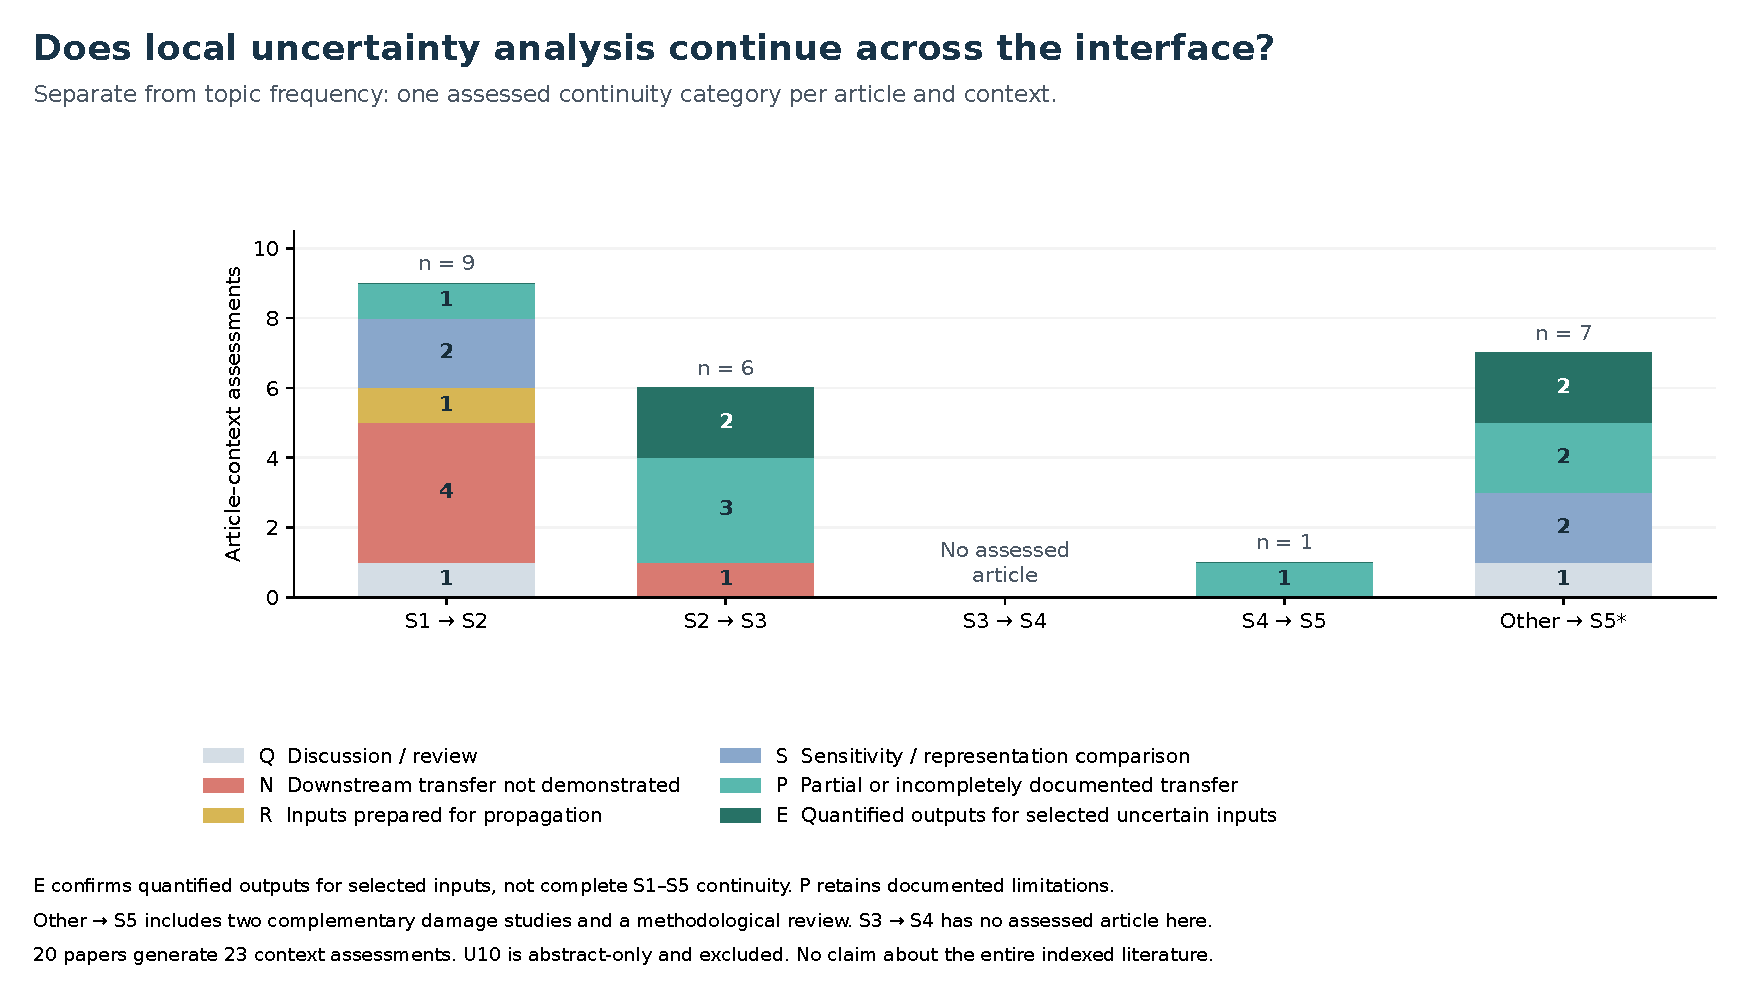
\includegraphics[width=\textwidth]{content_profiles/figures/03_continuity_evidence.pdf}
  \caption{Context-specific continuity assessments derived from archived evidence extraction. Each article--context pair has one assessment category. Quantified outputs for selected uncertain inputs do not demonstrate complete S1--S5 continuity. Methodological and complementary evidence retain their separate roles in the accompanying CSV. This figure does not constitute a new independent full-text review or a final PRISMA inclusion count.}
  \label{fig:content-continuity}
\end{figure}
.
% Requires \usepackage{graphicx}. Descriptive synthesis of archived extraction.
\begin{figure}[p]
  \centering
  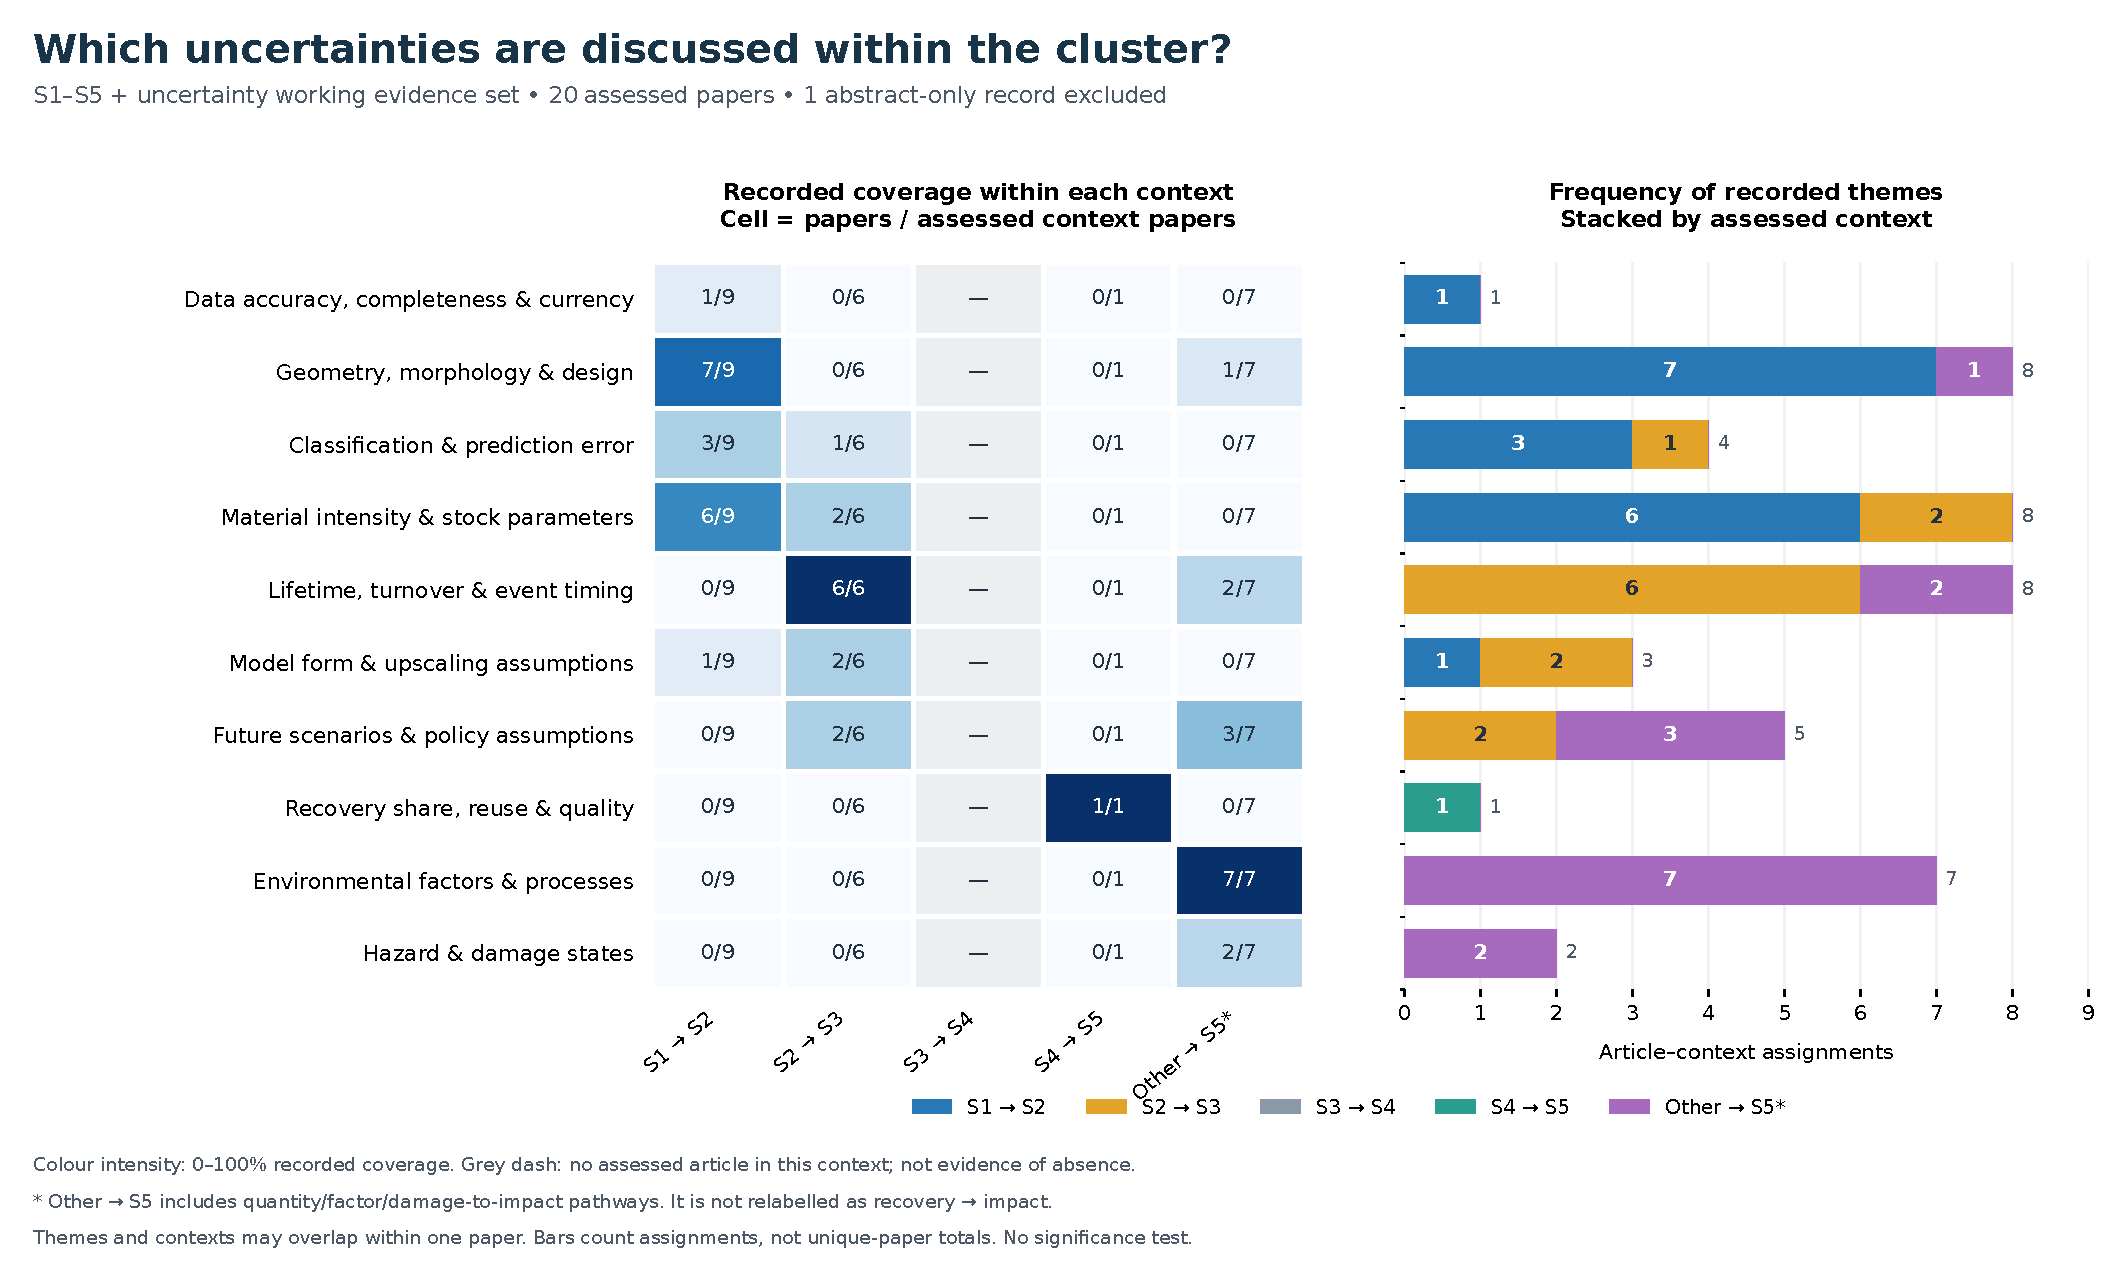
\includegraphics[width=\textwidth]{content_profiles/figures/01_uncertainty_sources.pdf}
  \caption{Recorded uncertainty sources within the S1--S5 uncertainty working set. Cells show papers with a recorded theme divided by assessed papers in each transition context. Twenty papers yield 23 article--context assessments; an abstract-only record is excluded. Themes and contexts may overlap. The grey column denotes no assessed article, not absence in the wider literature. The other-to-S5 group includes factor-, quantity- and damage-to-impact pathways and must not be interpreted as recovery-to-impact evidence.}
  \label{fig:content-uncertainty-sources}
\end{figure}

\begin{figure}[p]
  \centering
  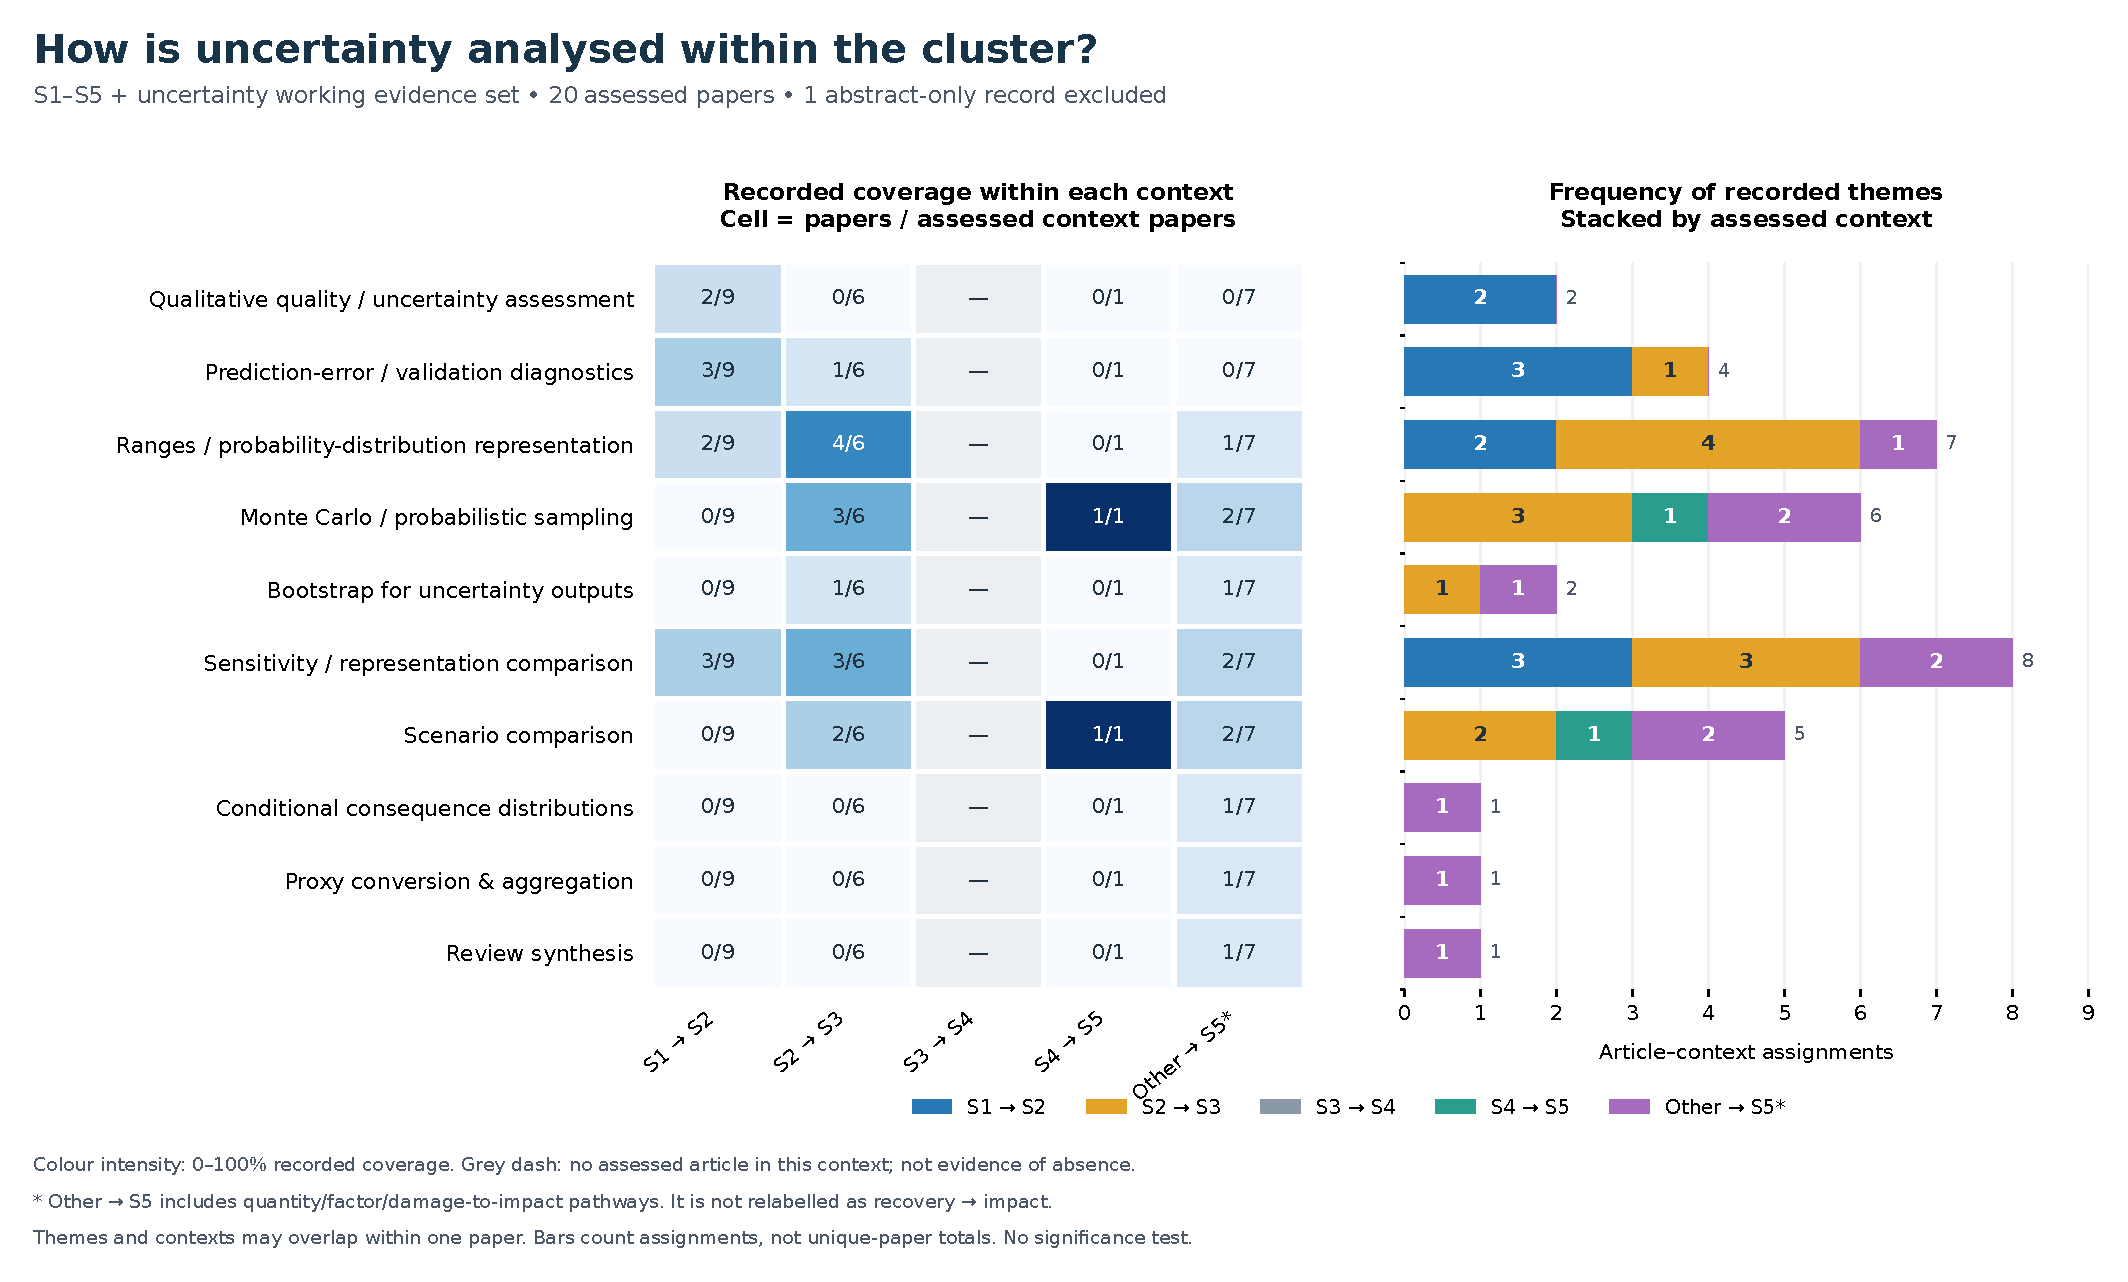
\includegraphics[width=\textwidth]{content_profiles/figures/02_uncertainty_methods.pdf}
  \caption{Recorded uncertainty-analysis methods in the same working set. Heatmap intensities are descriptive within-context proportions. Stacked frequencies count article--context assignments, not independent observations or unique-paper totals. A method's presence does not establish interstage uncertainty continuity. No inferential significance test is applied.}
  \label{fig:content-uncertainty-methods}
\end{figure}

\begin{figure}[p]
  \centering
  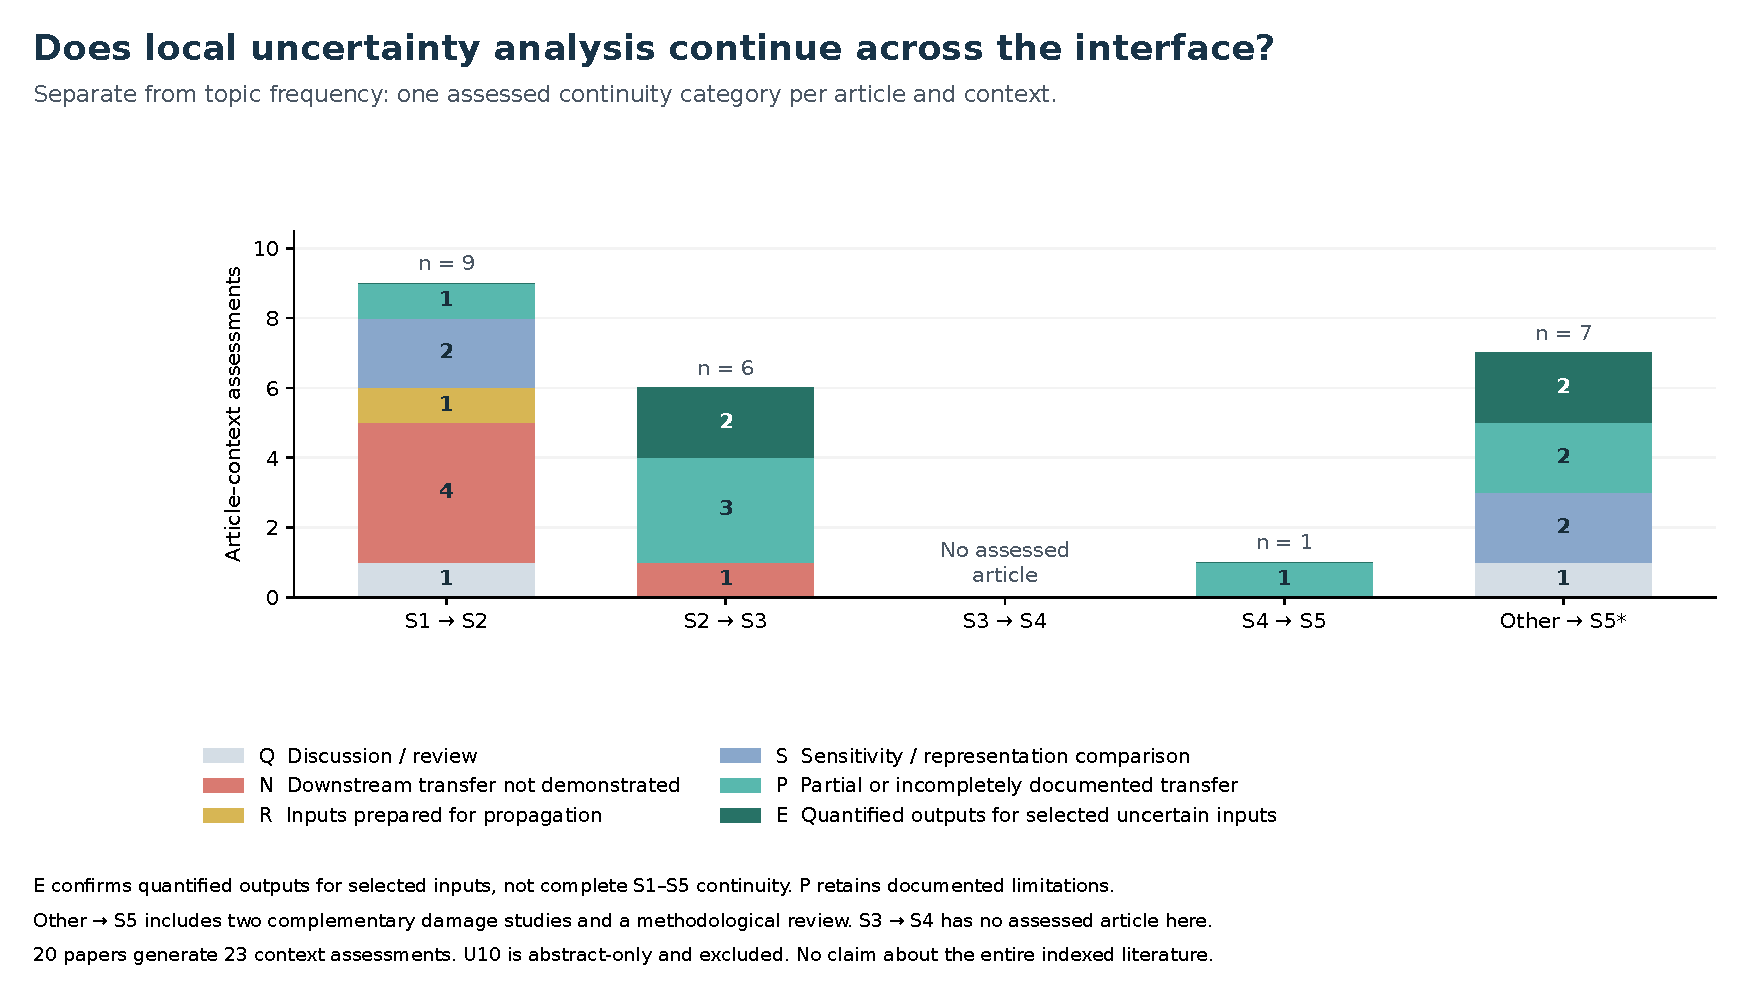
\includegraphics[width=\textwidth]{content_profiles/figures/03_continuity_evidence.pdf}
  \caption{Context-specific continuity assessments derived from archived evidence extraction. Each article--context pair has one assessment category. Quantified outputs for selected uncertain inputs do not demonstrate complete S1--S5 continuity. Methodological and complementary evidence retain their separate roles in the accompanying CSV. This figure does not constitute a new independent full-text review or a final PRISMA inclusion count.}
  \label{fig:content-continuity}
\end{figure}
.
% Requires \usepackage{graphicx}. Descriptive synthesis of archived extraction.
\begin{figure}[p]
  \centering
  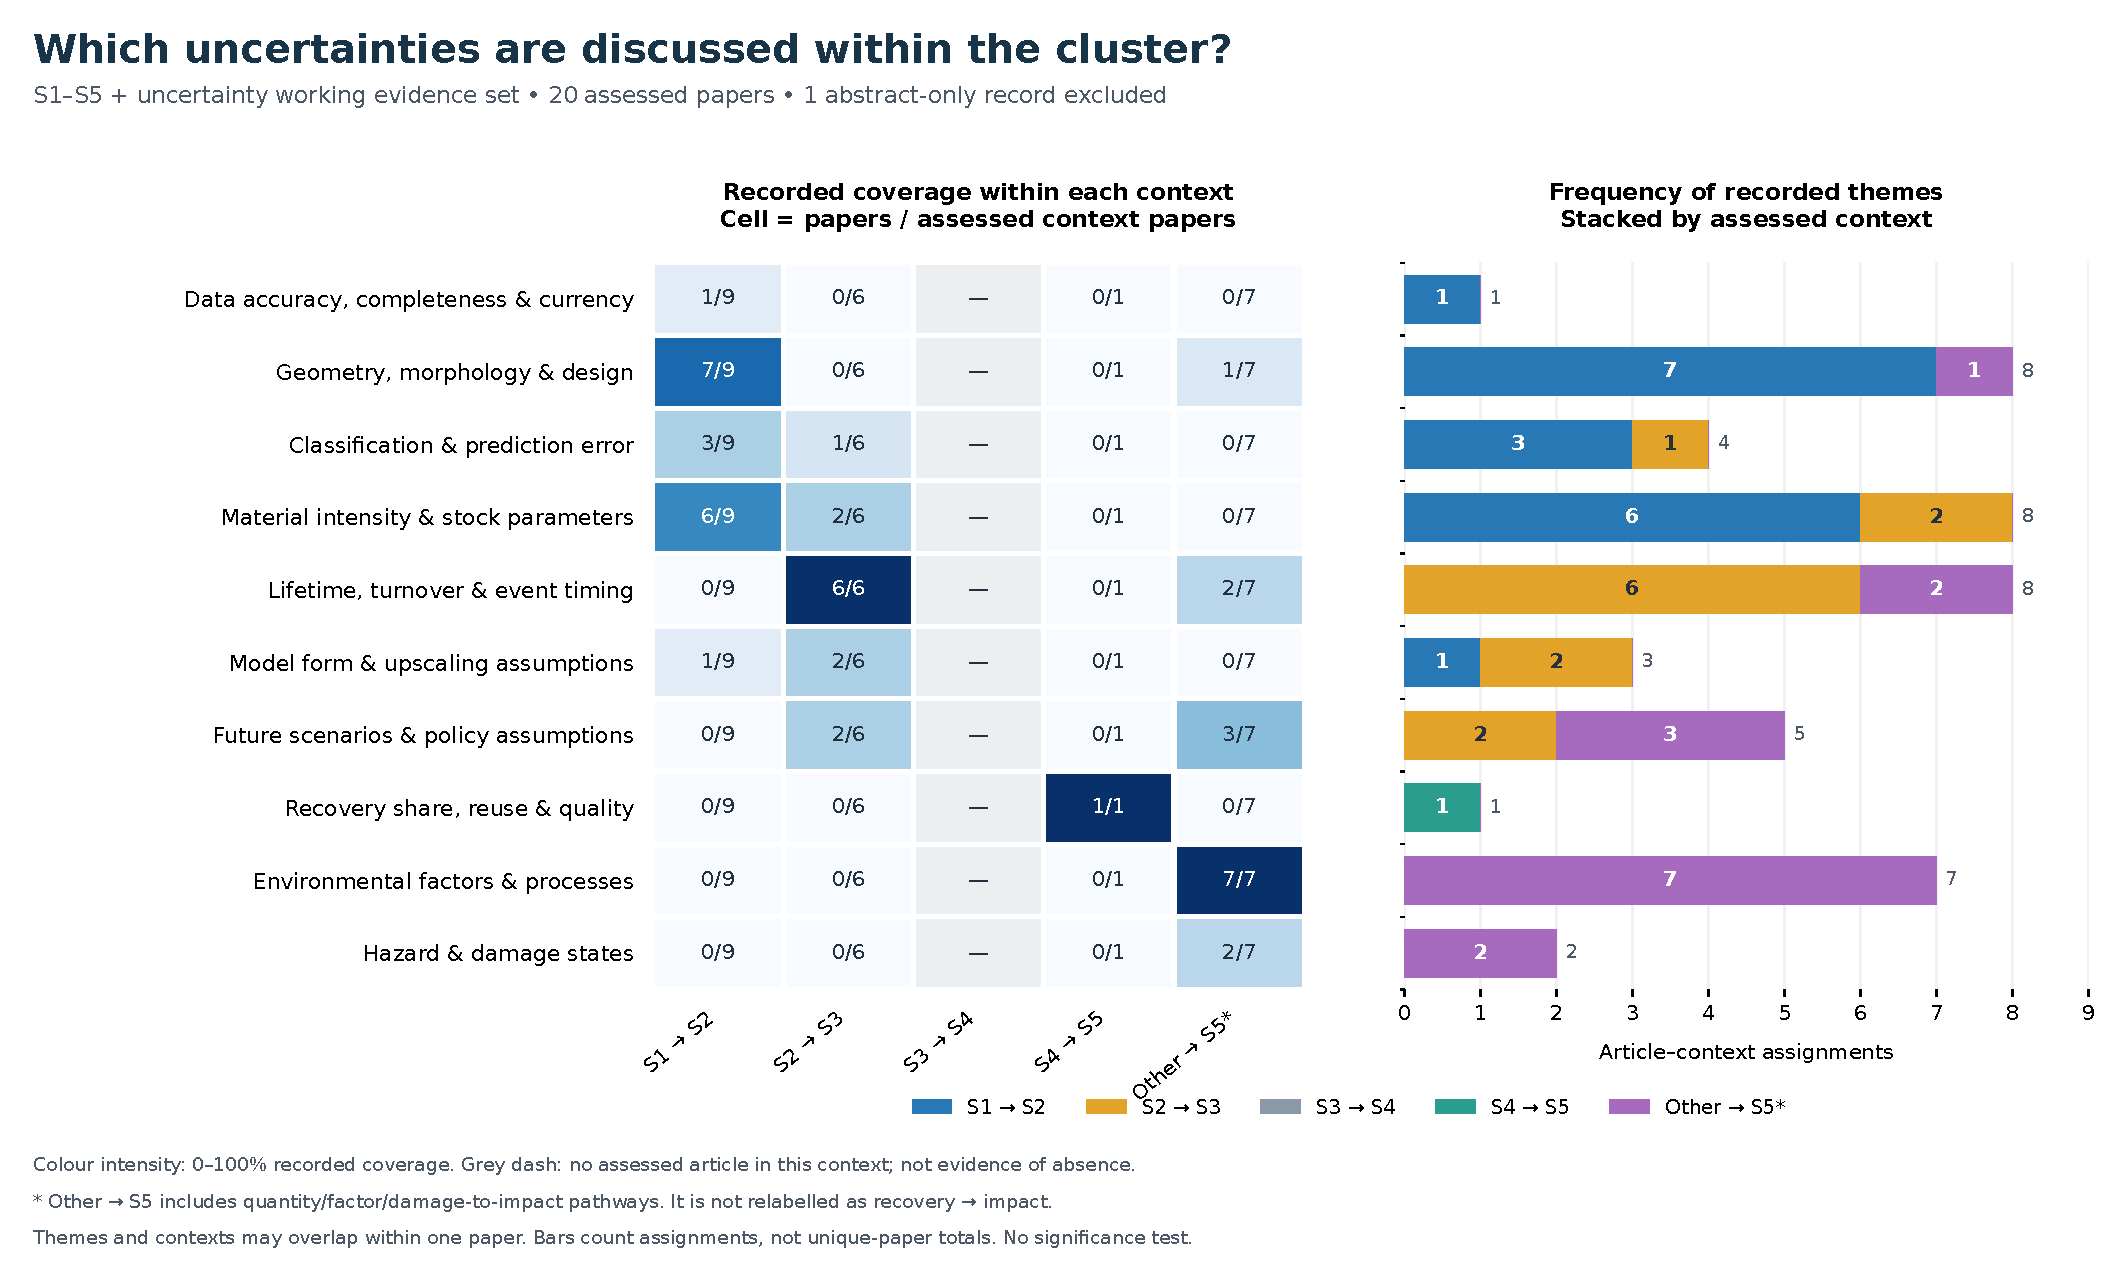
\includegraphics[width=\textwidth]{content_profiles/figures/01_uncertainty_sources.pdf}
  \caption{Recorded uncertainty sources within the S1--S5 uncertainty working set. Cells show papers with a recorded theme divided by assessed papers in each transition context. Twenty papers yield 23 article--context assessments; an abstract-only record is excluded. Themes and contexts may overlap. The grey column denotes no assessed article, not absence in the wider literature. The other-to-S5 group includes factor-, quantity- and damage-to-impact pathways and must not be interpreted as recovery-to-impact evidence.}
  \label{fig:content-uncertainty-sources}
\end{figure}

\begin{figure}[p]
  \centering
  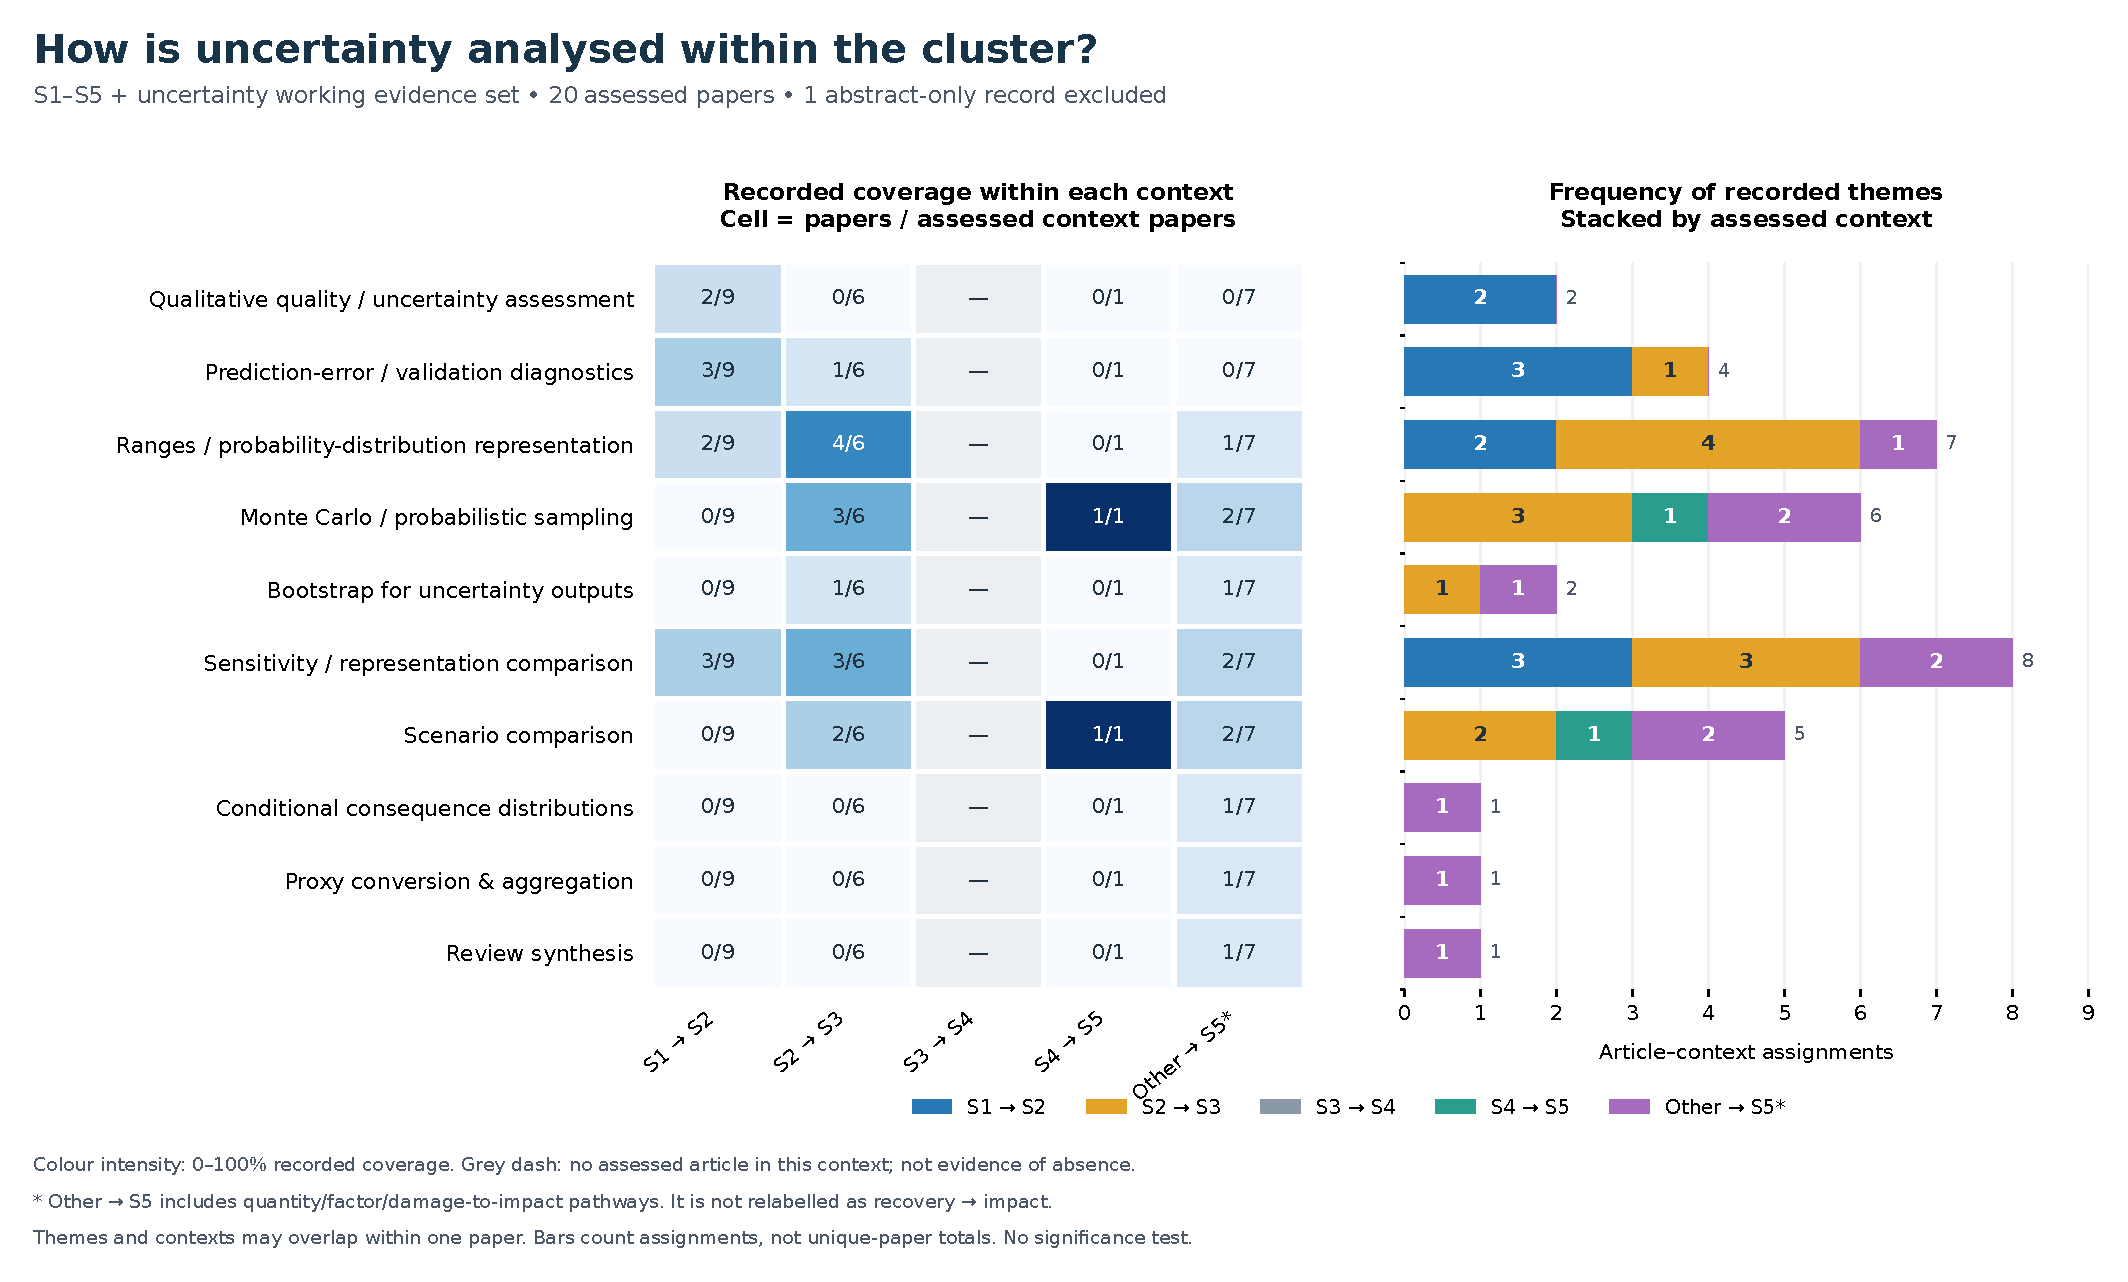
\includegraphics[width=\textwidth]{content_profiles/figures/02_uncertainty_methods.pdf}
  \caption{Recorded uncertainty-analysis methods in the same working set. Heatmap intensities are descriptive within-context proportions. Stacked frequencies count article--context assignments, not independent observations or unique-paper totals. A method's presence does not establish interstage uncertainty continuity. No inferential significance test is applied.}
  \label{fig:content-uncertainty-methods}
\end{figure}

\begin{figure}[p]
  \centering
  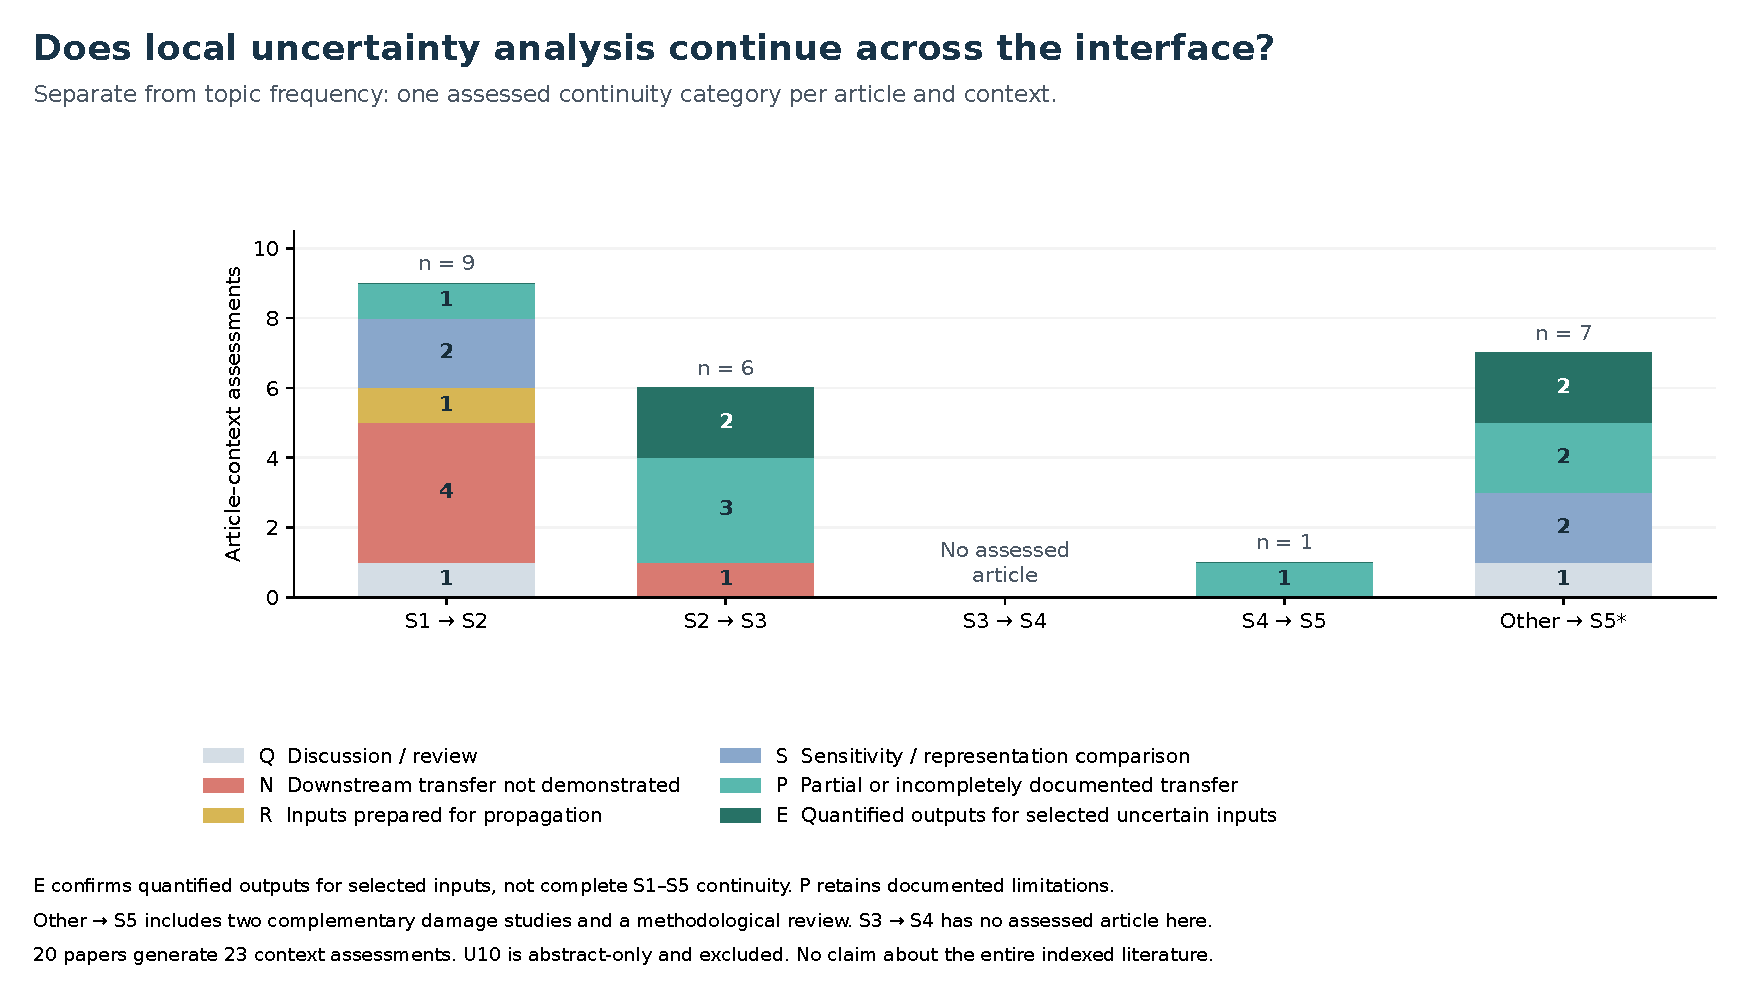
\includegraphics[width=\textwidth]{content_profiles/figures/03_continuity_evidence.pdf}
  \caption{Context-specific continuity assessments derived from archived evidence extraction. Each article--context pair has one assessment category. Quantified outputs for selected uncertain inputs do not demonstrate complete S1--S5 continuity. Methodological and complementary evidence retain their separate roles in the accompanying CSV. This figure does not constitute a new independent full-text review or a final PRISMA inclusion count.}
  \label{fig:content-continuity}
\end{figure}
